\documentclass[border=3pt,tikz]{standalone}
% Shared look for every TikZ figure in these notes.
% Included by each standalone figure file; also keeps the figures consistent
% with the colours used in the PDF and on the website.

\usepackage{tikz}
\usepackage{pgfplots}
\pgfplotsset{compat=1.18}
\usetikzlibrary{arrows.meta, decorations.markings, decorations.pathmorphing,
                patterns, calc, positioning}
\usepackage{amsmath}

% Series colours are the three validated categorical slots also used by the
% interactive widgets, so a path drawn in the printed notes and the same path on
% the website are the same colour. They clear the colour-vision-deficiency and
% contrast checks as a set; every path is direct-labelled as well, so colour is
% never the only thing carrying identity.
\definecolor{duPurple}{HTML}{68246D}
\definecolor{duBlue}{HTML}{2A78D6}
\definecolor{duRed}{HTML}{EB6834}
\definecolor{duGreen}{HTML}{1BAF7A}
\definecolor{duGrey}{HTML}{4D4D4D}

\tikzset{
  % heavier default lines and arrow tips, so diagrams stay clear when zoomed
  every picture/.append style = {line width=0.7pt, >={Stealth[length=3mm]}},
  axisline/.style   = {-{Stealth[length=3.4mm]}, line width=1.0pt, black},
  path1/.style      = {duBlue,   line width=1.6pt},
  path2/.style      = {duRed,    line width=1.6pt},
  path3/.style      = {duGreen,  line width=1.6pt},
  statedot/.style   = {circle, fill=black, inner sep=1.8pt},
  arrowhead/.style  = {decoration={markings,
                        mark=at position #1 with {\arrow{Stealth[length=3.4mm]}}},
                       postaction={decorate}},
  lbl/.style        = {font=\normalsize},
  slbl/.style       = {font=\small, duGrey},
  workfill/.style   = {duPurple, opacity=0.16},
}

% larger labels in plots as well
\pgfplotsset{every axis/.append style={label style={font=\normalsize}, tick label style={font=\small}, line width=0.9pt}}

% Boiler (358 x 379 px) with the water tubes taken as the control volume, and a
% condenser (354 x 256 px); both textbook images, labelled as on the board.
\begin{document}
\begin{tikzpicture}
  \node[anchor=south west, inner sep=0] (boil) at (0,0)
    {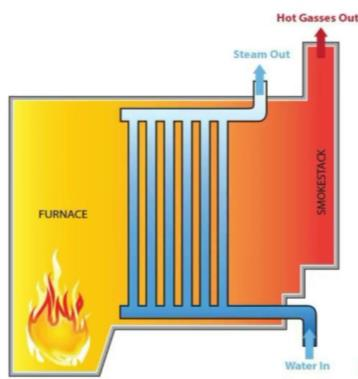
\includegraphics[height=5cm]{../img/ch4-heat-exchangers-boiler-clean.png}};
  \begin{scope}[shift={(boil.north west)}, x=5cm/379, y=-5cm/379]
    \draw[duGreen!80!black, dashed, line width=1.4pt, rounded corners=3pt,
          preaction={draw=white, solid, line width=2.6pt}]
      (115,119) rectangle (230,307);
  \end{scope}
  \node[anchor=south west, inner sep=0] (cond) at (5.9,0)
    {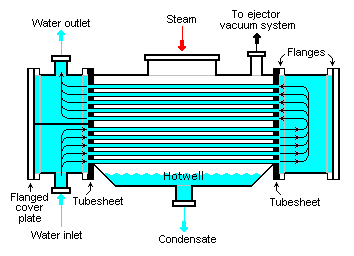
\includegraphics[width=7.6cm]{../img/ch4-heat-exchangers-condenser-clean.png}};
  \node[anchor=north, text=duRed, font=\normalsize] at ([yshift=-4pt]boil.south)
    {Boiler, $\dot{Q} > 0$};
  \node[anchor=north, text=duBlue, font=\normalsize] at ([yshift=-4pt]cond.south |- boil.south)
    {Condenser, $\dot{Q} < 0$};
\end{tikzpicture}
\end{document}
